\documentclass[a4paper,12pt]{article}
\usepackage{graphicx}
\usepackage[backend=biber]{biblatex}
\usepackage{float}
\usepackage[english]{babel}
\usepackage[titletoc]{appendix}
\usepackage{listings}
\usepackage{courier}

\lstset{basicstyle=\footnotesize\ttfamily,breaklines=true}

\addbibresource{bibliography.bib}
\usepackage[utf8]{inputenc}
\usepackage[T1]{fontenc}
\usepackage{times}
\usepackage{ifthen}
\usepackage[margin=25mm]{geometry}
\usepackage{fancyhdr}
\pagestyle{fancy}
\setlength{\parindent}{0pt}
\setlength{\parskip}{1ex plus 0.5ex minus 0.2ex}
\newcommand{\twodigit}[1]{\ifthenelse{#1<10}{0}{}{#1}}
\newcommand{\dagensdatum}{\number\year-\twodigit{\number\month}-\twodigit{\number\day}}

%% ------------------------------------------
% NYBILD
% Skapar centrerad bild med caption
%
% #1: Filens url relativt '/images/'
% #2: Caption
% #3: Label
% #4: Skalning
%% ------------------------------------------
\newcommand{\nyBild}[4]{
    \begin{figure}[H]
        \centering
        \includegraphics[angle=0,scale=#4]{images/#1}
        \caption{#2}
        \label{fig:#3}
    \end{figure}
}

%%  Redefinitions of commands containing @
\makeatletter
\makeatother

\newcommand{\LIPStitelsida}{
    {\ }\vspace{45mm}
    \begin{center}
        \textbf{\Huge \LIPSdokumenttyp}
    \end{center}
    \begin{center}
        {\large Alexander Vevstad, Amanda Aasa, Amanda Svennblad, \\Daniel Thomas, Lina Larsson, Olav Berg}
    \end{center}
    \begin{center}
        {\large \textbf{Version \LIPSversion}}
    \end{center}
    \begin{center}
        {Parts of chapter \ref{ch:intro} and \ref{ch:install} are based on the 2019 user guide for ENVISIoN.}
    \end{center}
    \vfill
    \begin{center}{
        \large Status}\\[1.5ex]
        \begin{tabular}{|*{3}{p{40mm}|}}
            \hline
            Granskad & \LIPSgranskare & \LIPSgranskatdatum \\
            \hline
            Godkänd & \LIPSgodkannare & \LIPSgodkantdatum \\
            \hline
        \end{tabular}
    \end{center}
}


\newenvironment{LIPSdokumenthistorik}{
    \begin{center}
        Document history\\[1ex]
        \begin{small}
            \begin{tabular}{|l|l|p{60mm}|l|l|}
                \hline
                \textbf{Version} & \textbf{Date} & \textbf{Changes} &
                \textbf{Done by} & \textbf{Reviewed} \\
                }
                {
                \hline
            \end{tabular}
        \end{small}
    \end{center}
}


\newcommand{\LIPSversionsinfo}[5]{\hline {#1} & {#2} & {#3} & {#4} & {#5} \\}
\newcounter{LIPSkravnummer}
\newcounter{LIPSunderkravnummer}[LIPSkravnummer]

\newenvironment{LIPSkravlista}{
    \begin{tabular}{|p{25mm}|p{25mm}|p{85mm}|p{5mm}|}
        }
        {
        \hline
    \end{tabular}
}

\newenvironment{LIPSleveranslista}{
    \begin{tabular}{|p{25mm}|p{15mm}|p{70mm}|p{25mm}|p{5mm}|}
        }
        {
        \hline
    \end{tabular}
}

\newenvironment{tabellexlista}{
    \begin{tabular}{|p{25mm}|p{25mm}|p{70mm}|p{20mm}|}
        }
        {
        \hline
    \end{tabular}
}

\newenvironment{dokumentlista}{
    \begin{tabular}{|p{28mm}|p{17mm}|p{39mm}|p{28mm}|p{28mm}|}
        }
        {
        \hline
    \end{tabular}
}

\newcommand{\dokumenttext}[5]{
    \hline 
    {#1} & {#2} & {#3} & {#4} & {#5} \\
}


\newcommand{\LIPSkrav}[3]{
    \hline
    \stepcounter{LIPSkravnummer}
    \textbf{Krav nr \arabic{LIPSkravnummer}} & \textbf{{#1}} & {#2} & \textbf{{#3}} \\
}

\newcommand{\tabellex}[3]{
    \hline
    Krav nr x & {#1} & {#2} & {#3} \\
}

\newcommand{\LIPSleverans}[2]{
  {#1} & {#2} & \hline
}

\newcommand{\LIPSunderkrav}[3]{
    \hline\stepcounter{LIPSunderkravnummer}\textbf{Krav nr \arabic{LIPSkravnummer}\Alph{LIPSunderkravnummer}} & \textbf{{#1}} & {#2} & \textbf{{#3}} \\
}

\newenvironment{LIPSprojektidentitet}{%
{\ }\vspace{45mm}
\begin{center}
  {\Large PROJECT IDENTITY}\\[0.5ex]
  {\small
  \LIPSartaltermin, \LIPSprojektgrupp\\
  Faculty of Science and Engineering, Linköping University, IFM
  }
\end{center}
\begin{center}
  {\small Group members}\\
%  \begin{tabular}{|p{30mm}|p{40mm}|p{35mm}|p{45mm}|}
  \begin{tabular}{|l|p{45mm}|p{25mm}|l|}
    \hline
    \textbf{Name} & \textbf{Role} & \textbf{Phone nr.} & \textbf{E-mail} \\
    \hline
}%
{%
    \hline
  \end{tabular}
\end{center}
\begin{center}
  {\small
    \textbf{Website}: \LIPSgrupphemsida\\[1ex]
    \textbf{Client}: \LIPSkund\\
    \textbf{Contact person of client}: \LIPSkundkontakt\\
    \textbf{Course examintor}: \LIPSkursansvarig\\
    \textbf{Main supervisor}: \LIPShandledare\\
  }
\end{center}
\newpage
}
\newcommand{\LIPSgruppmedlem}[4]{\hline {#1} & {#2} & {#3} & {#4} \\}

\NewDocumentCommand\secpdf{somO{1}m}{
  \clearpage
  \thispagestyle{fancy}
  \addcontentsline{toc}{section}{#3}
  \includepdf[
    pages=#4,
    pagecommand={
      \IfBooleanTF{#1}{
        \section*{#3}}{
        \IfNoValueTF{#2}{
          \section{#3}}{
          \section[#2]{#3}}}},
    scale=.80
    ]
    {#5}
}

\newenvironment{LIPSlicens}{
    \begin{center}
    \large{Licens}
    \end{center}
}{}

\pagenumbering{roman}
\newcommand{\LIPSartaltermin}{2018/Spring}
\newcommand{\LIPSkursnamn}{TFYA75}

\newcommand{\LIPSprojekttitel}{Visualization of electron structures}

\newcommand{\LIPSprojektgrupp}{Group 2}
\newcommand{\LIPSgruppepost}{}
\newcommand{\LIPSdokumentansvarig}{Marian Brännvall}

\newcommand{\LIPSkund}{IFM, Linköpings universitet, 581\,83 Linköping}
\newcommand{\LIPSkundkontakt}{Rickard Armiento, 013-281249, rickard.armiento@liu.se}
\newcommand{\LIPSkursansvarig}{Per Sandström, 013-282902, persa@ifm.liu.se}
\newcommand{\LIPShandledare}{Johan Jönsson, 013-281176, johan.jonsson@liu.se}


\newcommand{\LIPSdokumenttyp}{User guide}
\newcommand{\LIPSredaktor}{Viktor Bernholtz}
\newcommand{\LIPSversion}{1.0}
\newcommand{\LIPSdatum}{\dagensdatum}

\newcommand{\LIPSgranskare}{DOK}
\newcommand{\LIPSgranskatdatum}{2018-05-25}
\newcommand{\LIPSgodkannare}{Rickard Armiento}
\newcommand{\LIPSgodkantdatum}{2018-05-28}

\usepackage[titletoc]{appendix}
\usepackage{hyperref}
\hypersetup{
    colorlinks,
    citecolor=black,
    filecolor=black,
    linkcolor=black,
    urlcolor=black
}

\begin{document}

\LIPStitelsida

\begin{LIPSprojektidentitet}
  \LIPSgruppmedlem{Anders Rehult}{Project leader (PL)}{076-3161206}{andre449@student.liu.se}
  \LIPSgruppmedlem{\LIPSdokumentansvarig}{Document manager (DOK)}{070-7280044}{marbr639@student.liu.se}
  \LIPSgruppmedlem{Andreas Kempe}{Secretary (SE)}{073-9796689}{andke133@student.liu.se}
  \LIPSgruppmedlem{Viktor Bernholtz}{Viktor Bernholtz (VB)}{073-0386030}{vikbe253@student.liu.se}
\end{LIPSprojektidentitet}

\tableofcontents{}
\newpage

\addcontentsline{toc}{section}{Document history}
\begin{LIPSdokumenthistorik}
  \LIPSversionsinfo{0.1}{2018-05-22}{First draft.}{Project group}{PL}
  \LIPSversionsinfo{0.2}{2018-05-25}{Second draft.}{Project group}{DOK}
  \LIPSversionsinfo{1.0}{2018-05-28}{Approved for version one.}{Project group}{DOK}
\end{LIPSdokumenthistorik}
\newpage

\addcontentsline{toc}{section}{Licens}
\begin{LIPSlicens}
  This documet is licensed as CC0, see appendix~\ref{ref:licens}. 
 
\end{LIPSlicens}

\newpage
\pagenumbering{arabic}

\section{Introduction}
ENVISIoN is an open source toolkit for electron visualisation.

ENVISIoN is implemented by using a modified verision of the Inviwo visualisation framework, developed at the Scientific Visualization Group at Linköpings universitet, LIU.


ENVISIoN has been developed as a part of the course TFYA75: Applied Physics - Bachelor's Project, given at Linköpings universitet, LiU.

The present version was developed during the spring term of 2018 by a project group consisting of: Anders Rehult, Marian Brännvall, Andreas Kempe and Viktor Bernholtz. Supervisor: Johan Jönsson; Requisitioner and co-supervisor: Rickard Armiento; Visualization expert: Rickard Englund; and Course examiner: Per Sandström. The work is based on a previous version by the project group taking the course in the spring term of 2017 consisting of: Josef Adamsson, Robert Cranston, David Hartman, Denise Härnström, Fredrik Segerhammar. Supervisor: Johan Jönsson; Requisitioner and co-supervisor: Rickard Armiento; Visualization expert: Peter Steneteg; and Course examiner: Per Sandström.


ENVISIoN provides a set of Python scripts that allow the user to:

\begin{itemize}
\item Read and parse output from electronic structure calculations made by the program VASP and storing the result in a structured HDF5 file.
\item Generate interactive Inviwo visualisation networks for common tasks when analyzing electronic structure calculations. Presently there is support for visualising the crystal structure of the unit cell of a material, electron localization function (ELF)-data, electronic charge density, and density of states - both total and partial.
The system also provides the ability to interconnect some of the networks mentioned above.
\end{itemize}

\section{How to build and run ENVISIoN}
These instructions show how to build Inviwo and ENVISIoN on Ubuntu
18.04 LTS.

\subsection{Install git}

Start by installing git, which will be used to fetch ENVISIoN in the
next step.

\begin{lstlisting}[frame = single, breaklines=true]
sudo apt install git
\end{lstlisting}

\subsection{Download ENVISIoN}

Go to your home folder and clone ENVISIoN from Github. This guide will
assume that both ENVISIoN and Inviwo will be placed directly under the
home folder.

\begin{lstlisting}[frame = single, breaklines=true]
cd
git clone https://github.com/rartino/ENVISIoN
\end{lstlisting}

\subsection{Prepare Inviwo using the ENVISIoN install script}

ENVISIoN provides an install script for Ubuntu 18.04 LTS. Executing
the installation script will install all required dependencies, clone
Inviwo from Github and configure the Inviwo build.

The script should \emph{NOT} be run as root, but as your own user and
it will ask for your password when it needs root rights. It is
possible that the script will ask for other user input during the
process, if that's the case, just accept the default.

\begin{lstlisting}[frame = single, breaklines = true]
cd ~/ENVISIoN/scripts

./install_envision_ubuntu_1804.sh /home/$USER/ENVISIoN /home/$USER/inviwo
\end{lstlisting}

Once the installation script has run, it prints build instructions.
Follow the instructions and start the build. The instructions will
tell you to \emph{cd} to the build directory and execute make.

An easy way to modify the build settings, if needed, is to install
the cmake curses gui and run it in the build directory.

To install the cmake gui:
\begin{lstlisting}[frame = single, breaklines = true]
sudo apt install cmake-curses-gui
\end{lstlisting}

Running cmake in the build directory:
\begin{lstlisting}[frame = single, breaklines = true]
cd ~/inviwo/build
ccmake .
\end{lstlisting}

When in the GUI, press \emph{c} to apply the current configuration,
\emph{g} to generate build files and \emph{q} to quit. If settings
have changed, it is possible that you will need to press \emph{c} more
than once before the \emph{g} option becomes available.

After having generated the build files, the project can now be rebuilt
with the new settings by executing \emph{make} like earlier.

\section{Start Inviwo and run ENVISIoN scripts}
After the Inviwo build is done, the binary will be available as
\emph{bin/inviwo} in the build folder. Start it by executing the
command below, while still standing in the build directory.

\begin{lstlisting}[frame = single, breaklines=true]
cd ~/inviwo/build
./bin/inviwo
\end{lstlisting}

\begin{itemize}
\item Open Python Editor under Python menu.
\item In the Python editor, click Open Script.
\item Select one of the scripts.
\item Click open.
\item Click the python logo in the top left corner to run.
\end{itemize}

More information about each script and how to use them in chapter \ref{ch:scripts}.

\section{Scripts}
\label{ch:scripts}
Descriptions and examples of all the avaliable scripts are found below. The scripts are called through the python editor in Inviwo as shown in figure \ref{fig:python_editor}.

\begin{figure} [H]
\centering
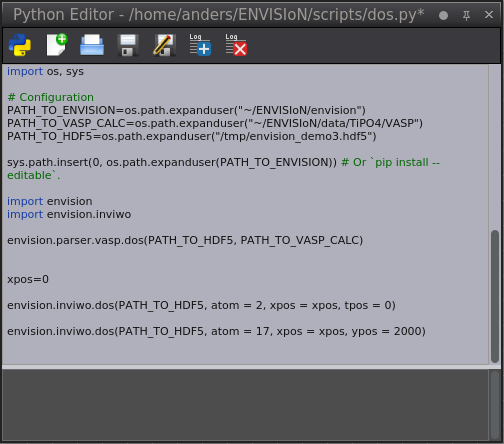
\includegraphics[scale=0.6]{screenshot_dos_script.png}
\caption{Python script for calling on the DOS visualisation module of ENVISIoN. Note that the pathway PATH\_TO\_VASP\_CALC here is set to "\textasciitilde/ENVISIoN/data/TiPO4/VASP", the folder containing the relevant VASP output files.}
\label{fig:python_editor}
\end{figure}
In all of the scripts the user has to specify the path to ENVISIoN, a path where VASP output files are found, and a desired path where ENVISIoN will generate a HDF5-file, or, if one already exists, use that file and skip parsing VASP data. \textbf{NOTE:} change the value of PATH\_TO\_HDF5, delete the HDF5-file, or rename the HDF5-file in between visualisations if a new material is to be visualised.

\subsection{Unit cell}
In the Python editor of Inviwo the user can choose to generate a visualisation of the unit cell by opening the folder \textit{scripts} and running the file \textit{unitcell.py}.

Figure \ref{fig:enhetscell} is an example of a unit cell visualisation, in this case of TiPO4. Figure \ref{fig:enhetscellnatverk} shows the network responsible for the aforementioned visualisation.
\begin{figure}[H]
    \centering
    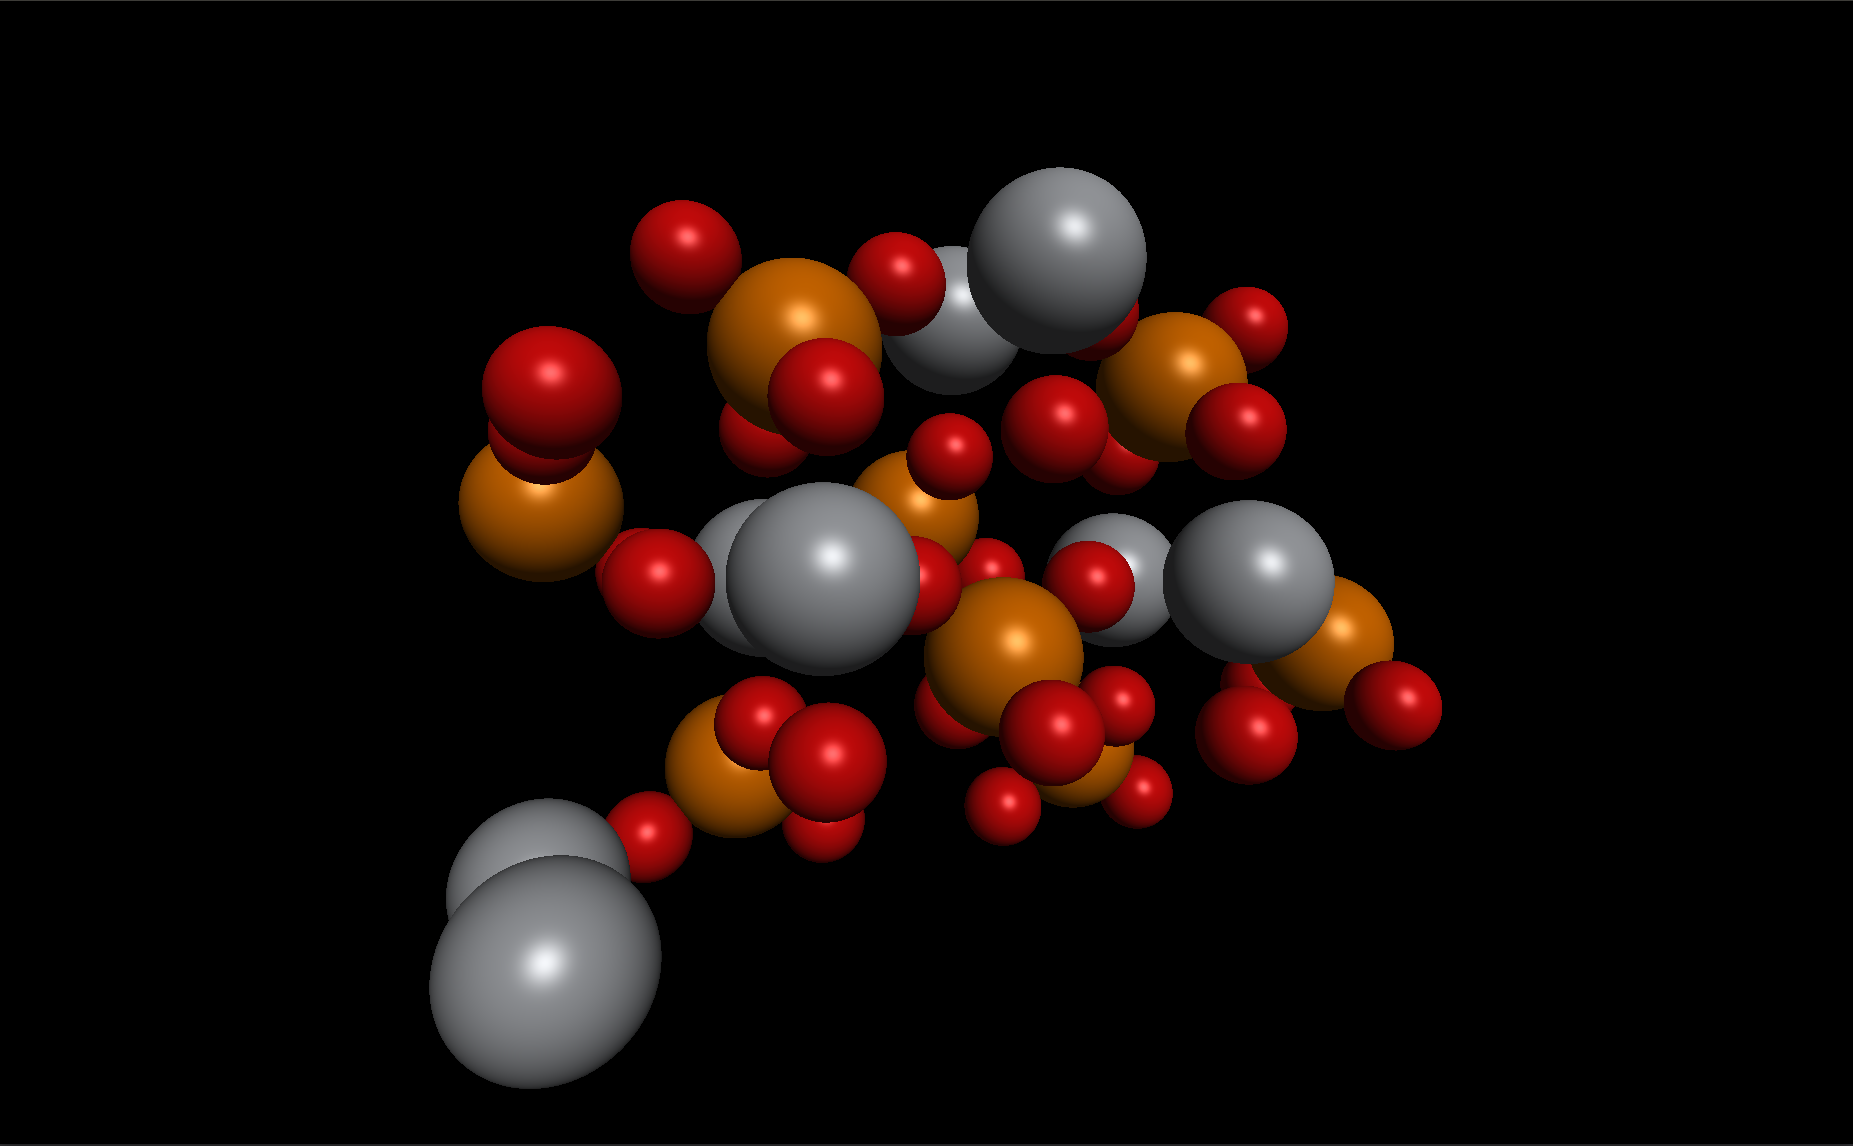
\includegraphics[scale=0.25]{screenshot_enhetscell_TiPO4.png}
    \caption{Visualisation of the crystal structure of the unit cell of TiPO4 in Inviwo.}
    \label{fig:enhetscell}
\end{figure}

\begin{figure}[H]
    \centering
    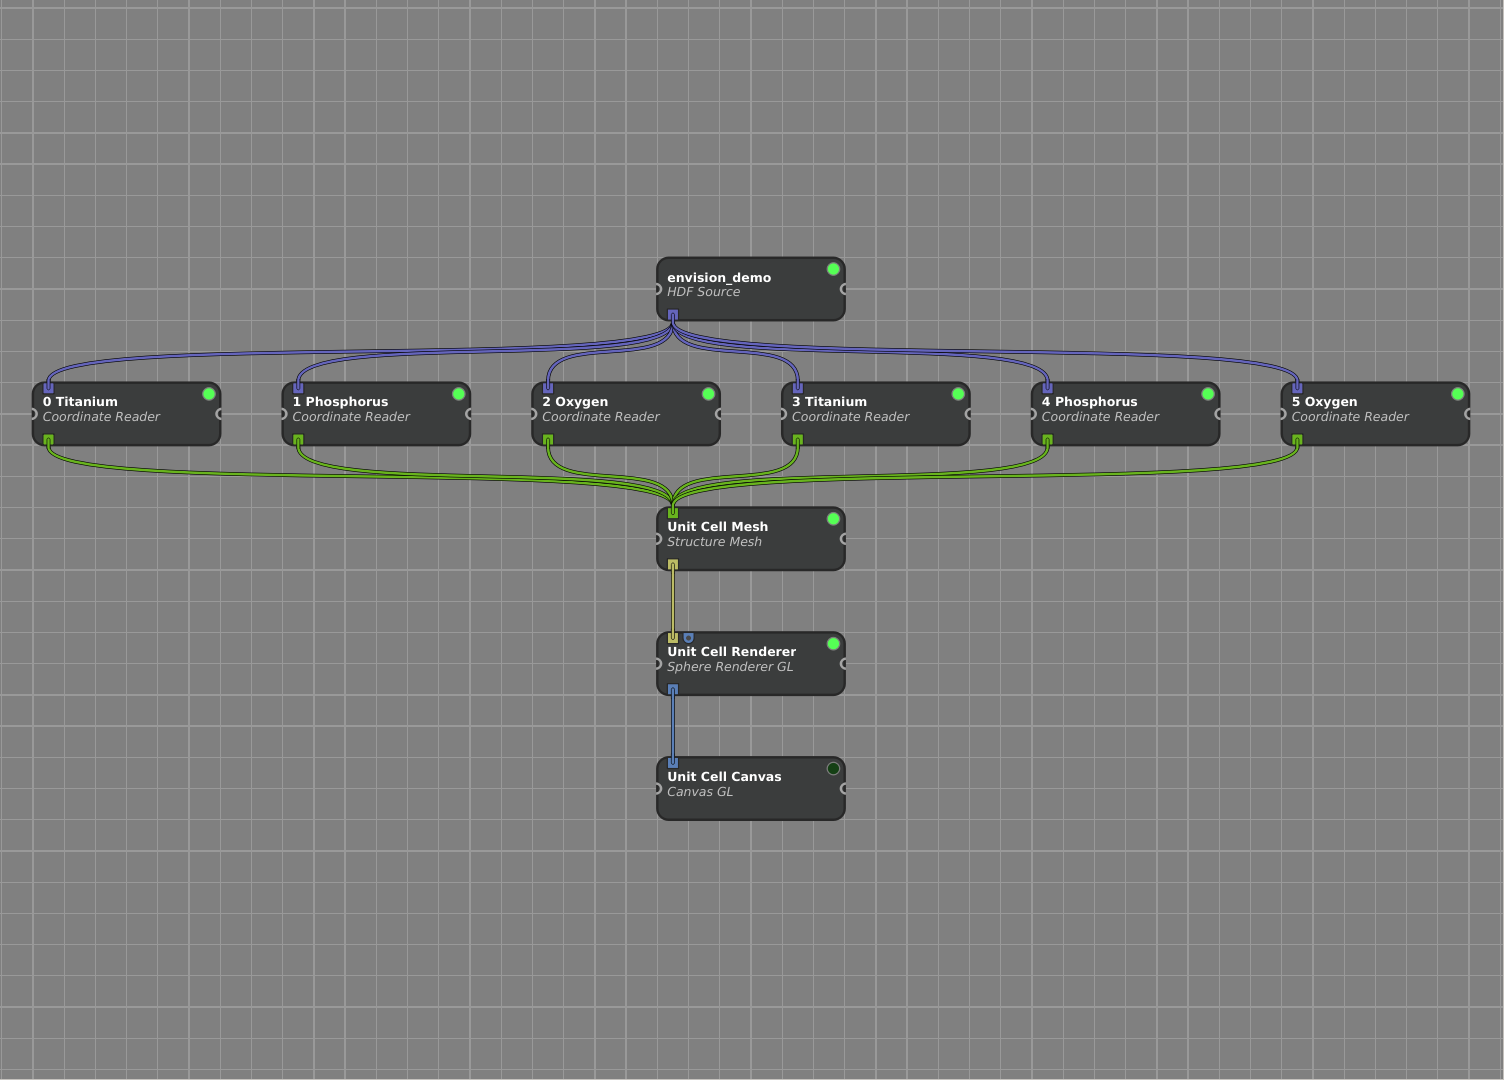
\includegraphics[scale=0.30]{screenshot_enhetscellnatverk_TiPO4.png}
    \caption{Network for visualisation of TiPO4 in Inviwo.}
    \label{fig:enhetscellnatverk}
\end{figure}

\subsection{ELF}
In the Python editor of Inviwo the user can choose to generate a visualisation of the Electron Localisation Function (ELF)-data as shown in figure \ref{fig:screenshot_elf} with corresponding network shown in figure \ref{fig:screenshot_elf_network} by opening the folder \textit{scripts} and running the file \textit{elf.py}. A second image showing the ELF-data of a slice of the unit cell can be added by changing the argument \textit{Slice} of the function \textit{elf} to True. This slice corresponds to a plane intersecting the unit cell, which can be moved using the W and S keys on the keyboard. The orientation of this plane can be changed by selecting the processor "Volume Slice" in the network by clicking on it, then choosing another value from the drop down menu in the property "Slice along axis".

The ELF-data can also be visualised as an isosurface. This is achieved by changing the argument \textit{iso} of the function \textit{elf} from None to any value between 0 and 1. The slice function described above is not compatible with isosurface visualisation.

The colors and opacities of different values can be changed by selecting the processor "ELF raycaster" in the network, clicking on the property "Transfer function", and interacting with the window that pops up. This window shows multicolored dots which can be manipulated to control opacity. Dots can be added by double clicking, and removed by clicking a dot and pressing the Delete key on the keyboard. Dots can be dragged and dropped using the mouse. The horizontal axis of the plane on which the dots are placed corresponds to ELF values between 0 and 1, while the vertical axis corresponds to opacities between 0 (transparent) and 1 (completely opaque). Figure \ref{fig:screenshot_transfer_function} in chapter \ref{ch:charge} shows what this window looks like.
\begin{figure} [H]
\centering
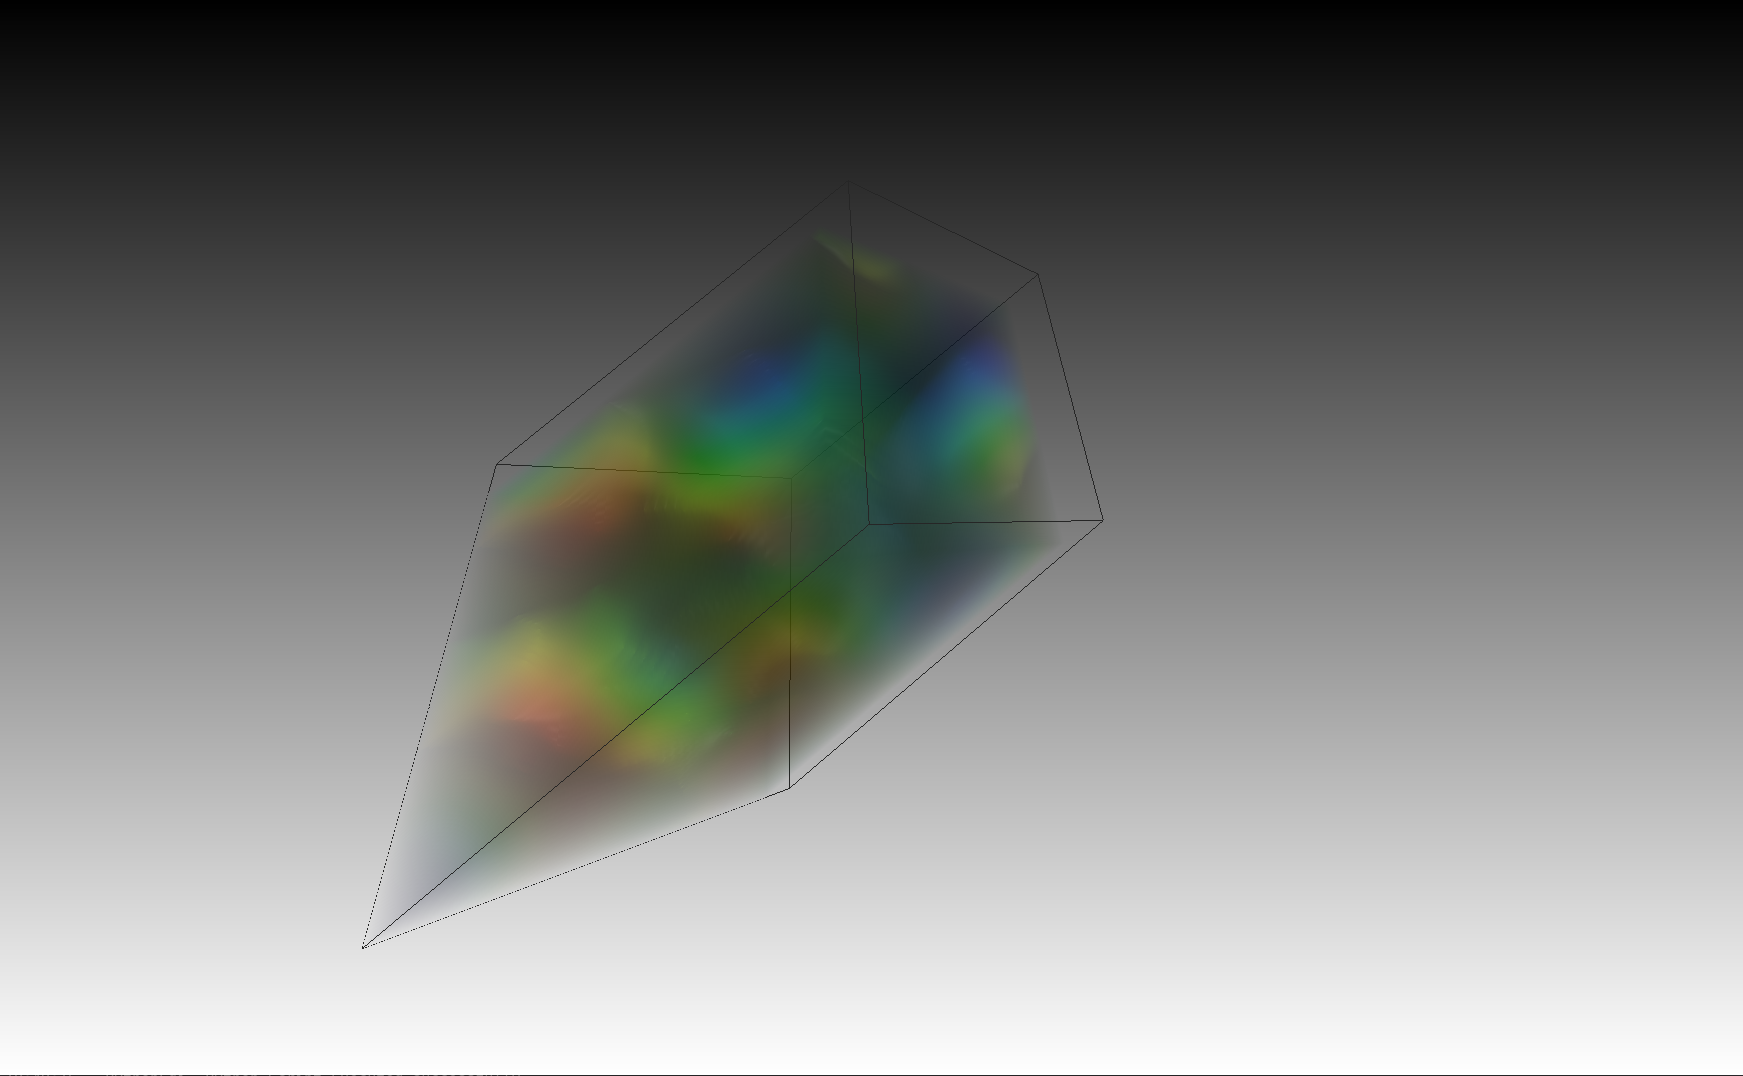
\includegraphics[scale = 0.20]{screenshot_elf_diamant.png}
\caption{Visualisation of ELF-data for diamond in Inviwo.}
\label{fig:screenshot_elf}
\end{figure}

\begin{figure} [H]
\centering
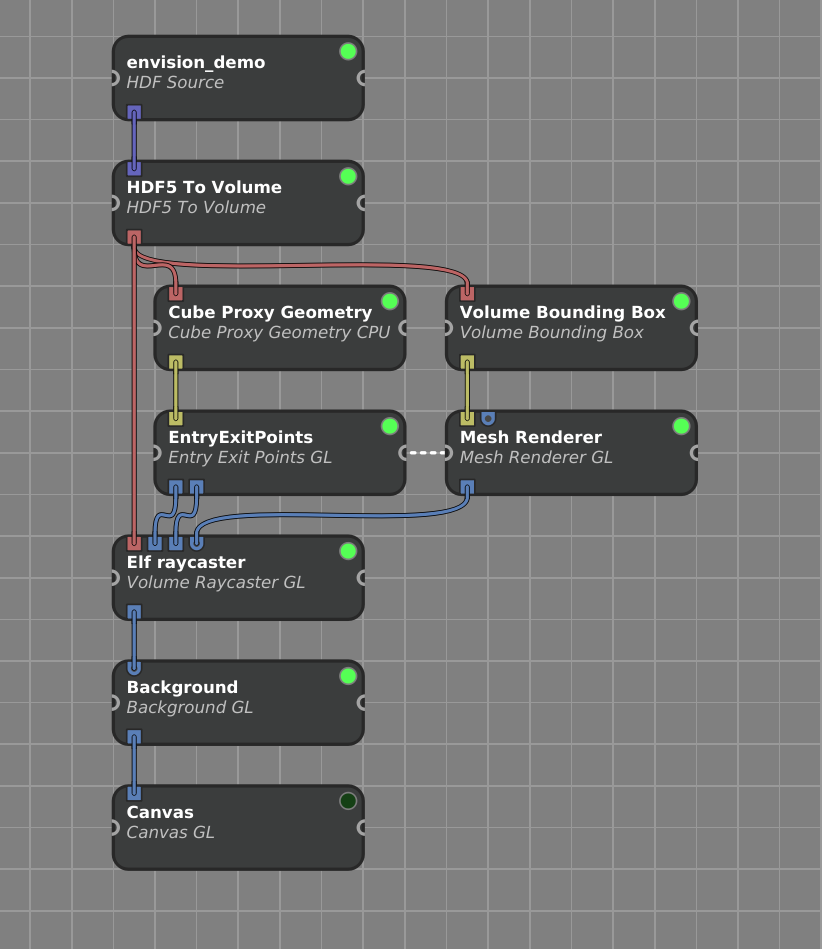
\includegraphics[scale=0.4]{screenshot_elfnatverk_diamant.png}
\caption{Network for visualisation of ELF-data for diamond in Inviwo.}
\label{fig:screenshot_elf_network}
\end{figure}

\subsection{Charge density}
\label{ch:charge}
In the Python editor of Inviwo the user can choose to generate a visualisation of the charge density by opening the folder \textit{scripts} and running the file \textit{charge.py}. A second image showing the charge density of a slice of the unit cell can be added by changing the argument \textit{Slice} of the function \textit{charge} to True. This slice corresponds to a plane intersecting the unit cell, which can be moved using the W and S keys on the keyboard. The orientation of this plane can be changed by selecting the processor "Volume Slice" in the network by clicking on it, then choosing another value from the drop down menu in the property "Slice along axis". This type of visualisation is shown in figure \ref{fig:screenshot_NaCl_laddningstathetslice}, and the generating network is found in figure \ref{fig:screenshot_NaCl_laddningstathetslicenatverk}.

The charge density can also be visualised as an isosurface. This is achieved by changing the argument \textit{iso} of the function \textit{charge} from None to any value between 0 and 1. Figure \ref{fig:screenshot_NaCl_laddningstathet_iso} shows an example of this. The slice function described above is not compatible with isosurface visualisation.

The colors and opacities of different values can be changed by selecting the processor "Charge raycaster" in the network, clicking on the property "Transfer function", and interacting with the window that pops up. This window shows multicolored dots which can be manipulated to control opacity. Dots can be added by double clicking, and removed by clicking a dot and pressing the Delete key on the keyboard. Dots can be dragged and dropped using the mouse. The horizontal axis of the plane on which the dots are placed corresponds to charge density values between 0 and 1, while the vertical axis corresponds to opacities between 0 (transparent) and 1 (completely opaque). Figure \ref{fig:screenshot_transfer_function} shows what this window looks like.

\begin{figure} [H]
\centering
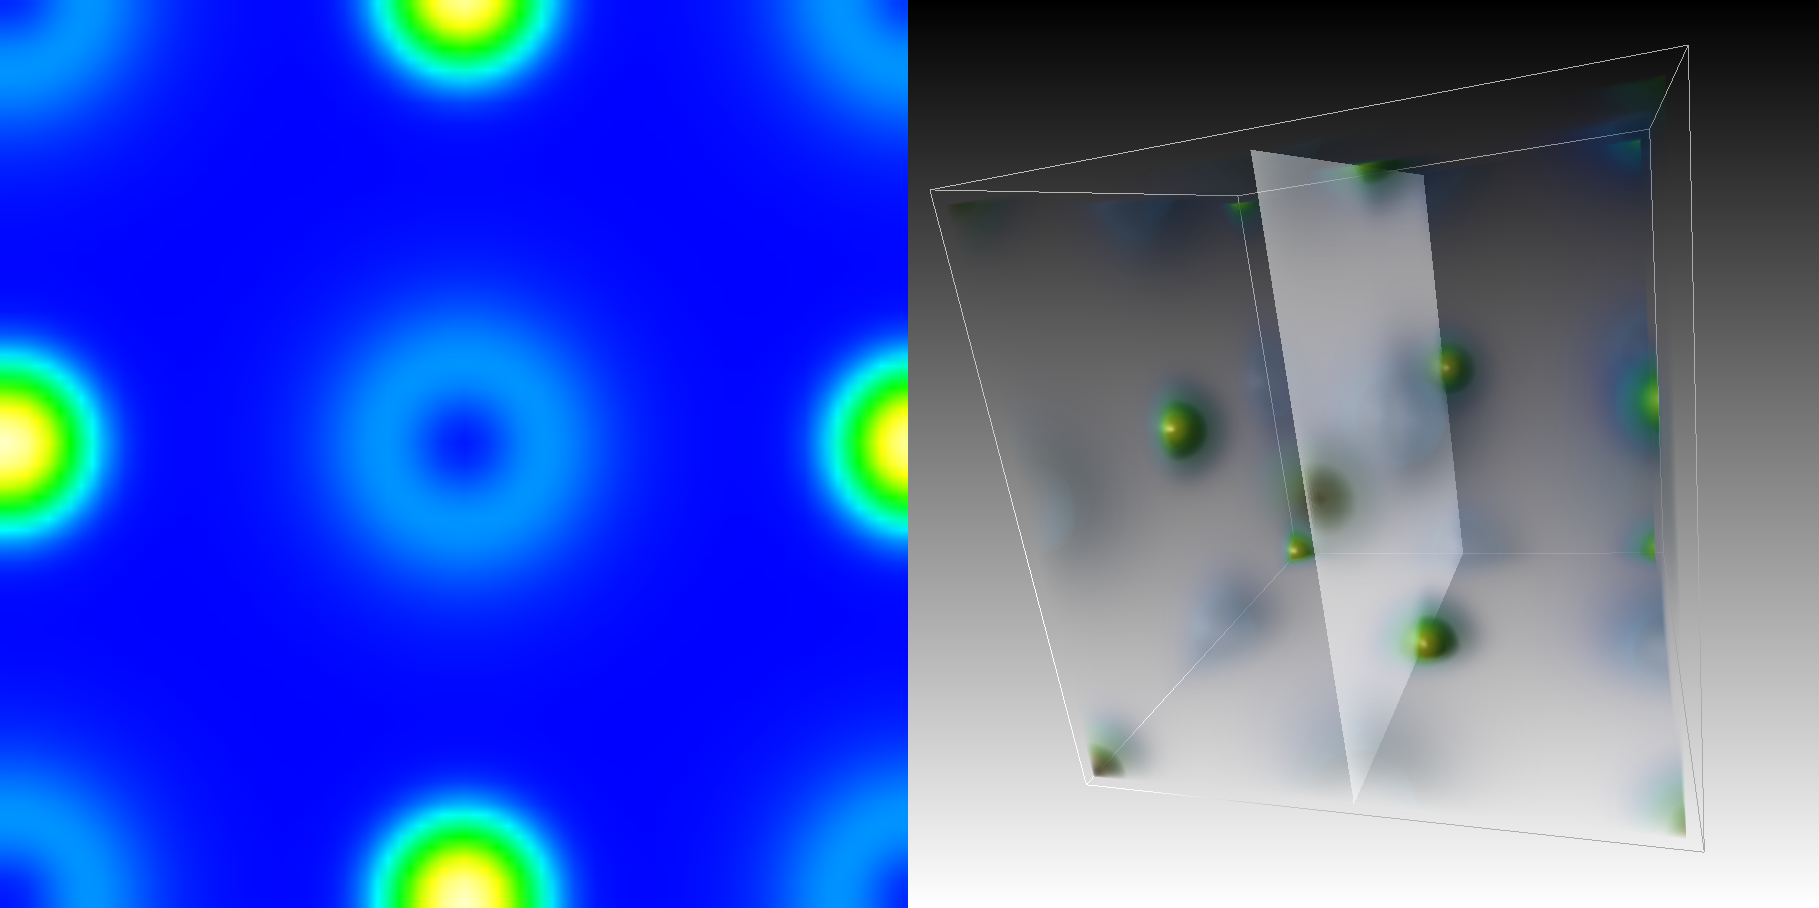
\includegraphics[scale=0.20]{screenshot_NaCl_laddningstathetslice.png}
\caption{Visualisation of charge density for NaCl with slice function in Inviwo.}
\label{fig:screenshot_NaCl_laddningstathetslice}
\end{figure}

\begin{figure} [H]
\centering
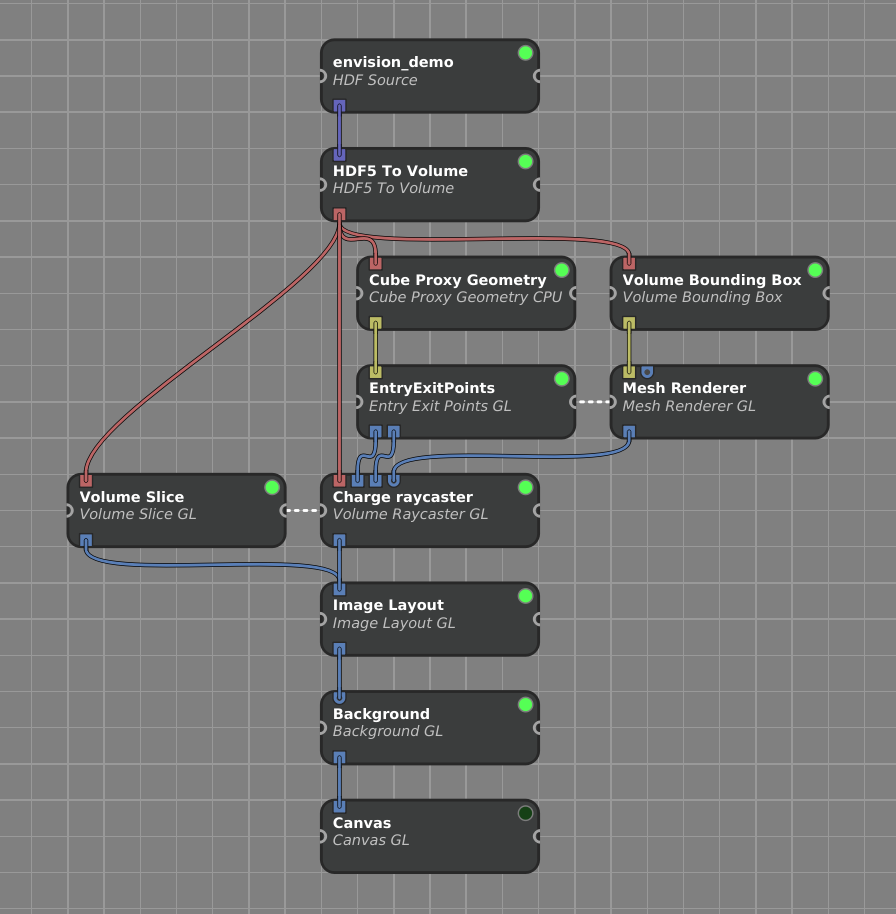
\includegraphics[scale=0.4]{screenshot_NaCl_laddningstathetslicenatverk.png}
\caption{Network for visualisation of charge density for NaCl with slice function in Inviwo.}
\label{fig:screenshot_NaCl_laddningstathetslicenatverk}
\end{figure}

\begin{figure} [H]
\centering
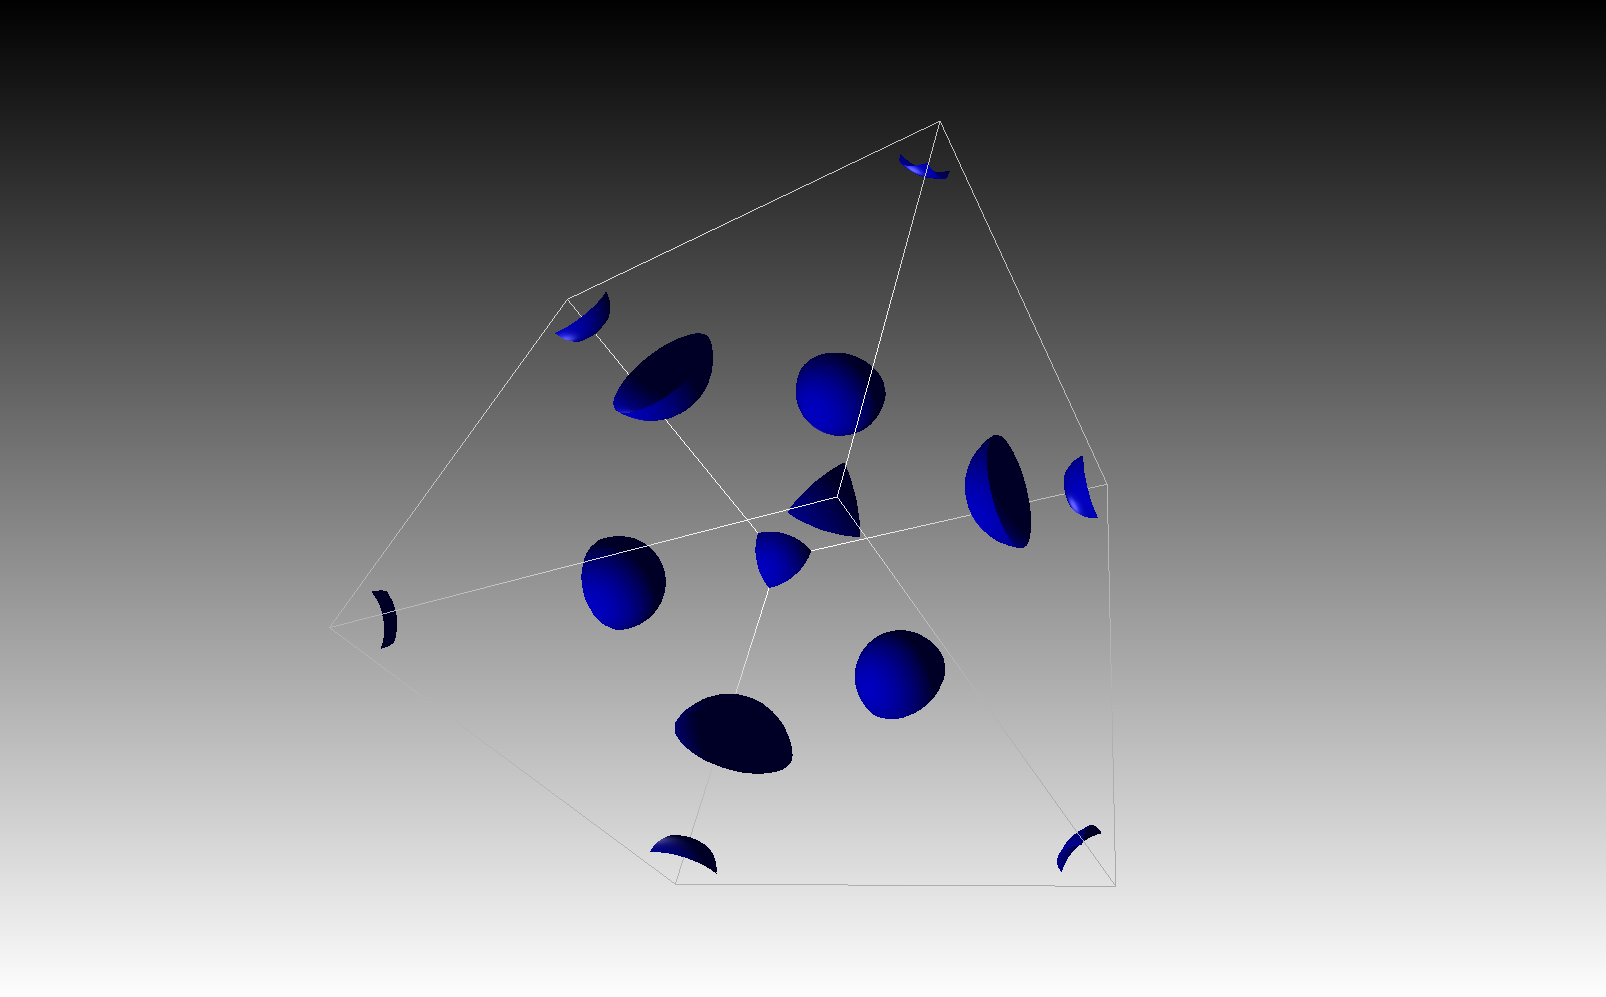
\includegraphics[scale=0.3]{screenshot_NaCl_laddningstathet_iso.png}
\caption{Visualisation of charge density for NaCl with ISO raycasting.}
\label{fig:screenshot_NaCl_laddningstathet_iso}
\end{figure}

\begin{figure} [H]
\centering
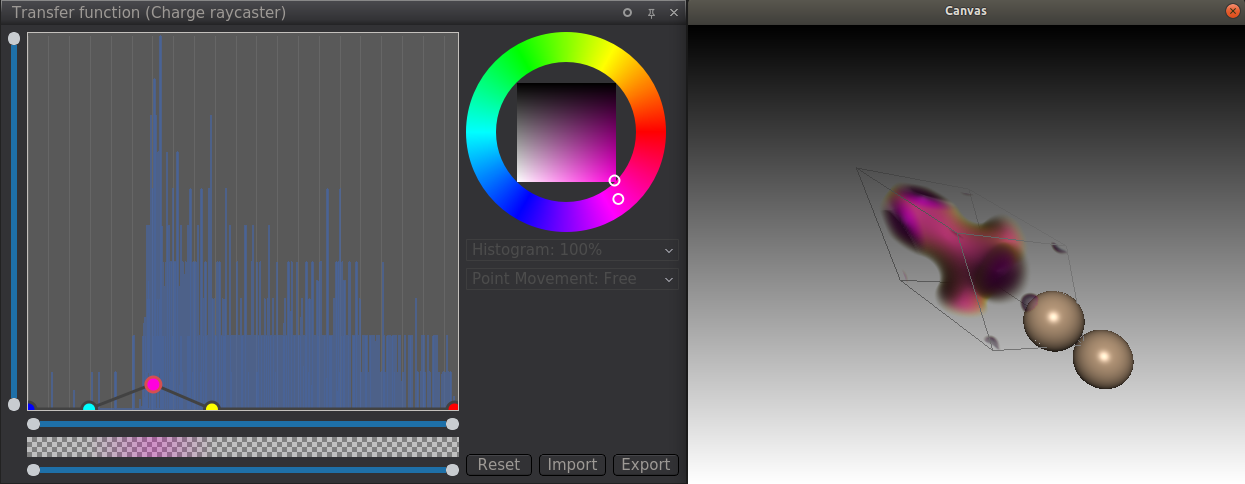
\includegraphics[scale=0.4]{screenshot_transfer_function_transparent.png}
\caption{Transfer function of the Charge raycaster processor and visualisation of charge density of Si connected with unit cell visualisation. Charge density values between 0.15 and 0.45 are illustrated as a somewhat transparent purple volume.}
\label{fig:screenshot_transfer_function}
\end{figure}

\subsection{Partial charge density}
In the Python editor in Inviwo, the user can choose to generate a visualisation of the band decomposed partial charge density by opening the folder \textit{scripts} and running the file \textit{parchg.py}.

When running the Python script, the user is required to specify what bands to visualise and how to visualise them. This is done by passing a list of the band numbers to the \textit{inviwo.parchg} function and then choosing one of the following modes:

\begin{itemize}
    \item \textbf{Total}: Display total partial charge density for all bands specified. 
    \item \textbf{Magnetic}: Display magnetic partial charge density for all bands specified. 
    \item \textbf{Up}: Display only the spin-up components of the charge density for all bands specified. 
    \item \textbf{Down}: Display only the spin-down components of the charge density for all bands specified. 
    \item \textbf{Mixed}: Use different modes for different bands as specified in the following list. 
\end{itemize}

If the \textit{mixed} mode is chosen, the user is required to pass another list to the function with the same length as the band list, where each element should be a number from  0 to 3 corresponding to the modes \textit{total}, \textit{magnetic}, \textit{up} and \textit{down} in that order. For example, if the band list given is [31, 212] and the mode list is [1, 3], band 31 will be visualized as in mode \textit{magnetic} and band 212 in mode \textit{down}.

After visualizing the partial charge density, the visualization can be manipulated in the same manner as described in section \ref{ch:charge}.

\subsection{DOS}
In the Python editor in Inviwo, the user can choose to generate a visualisation of the density of states by opening the folder \textit{scripts} and running the file \textit{dos.py}.

Figure \ref{fig:total_dos} is an example of a visualisation of the total density of states, in this case for Cu. Figure \ref{fig:network_dos} shows the network for the visualisation. This network generates both a 2D-graph of the total density of states and a similar graph but for the partial density of states. The partial density of states is by default shown for one atom, in two graphs for spin-polarized calculations, determined by the argument \textit{atoms} in the function \textit{dos}. See chapter \ref{ch:unitcell_dos} for a description of how to pick the atom for which to show projected DOS.

Visualisation of the partial DOS for one specific orbital (s, p, d, or f) of an atom can be achieved by deleting the connections between the undesired processors of type "HDF5 To Function" and the corresponding processor with name "Partial Add". To do this, select a connection by clicking on it and press the Delete key.

\begin{figure}[H]
    \centering
    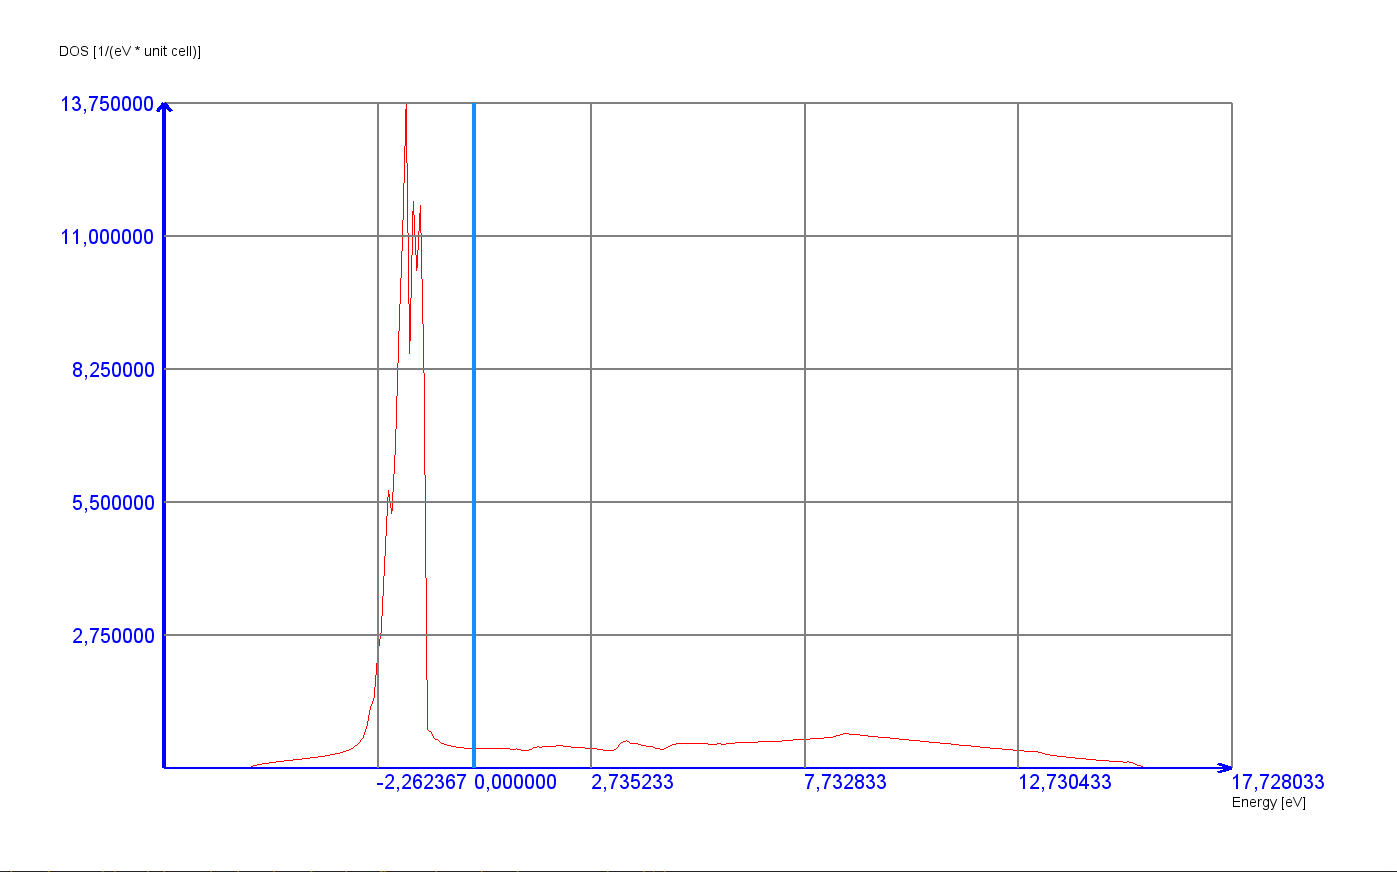
\includegraphics[scale=0.35]{screenshot_total_dos_Cu_1_10.png}
    \caption{Visualisation of total DOS for Cu.}
    \label{fig:total_dos}
\end{figure}

\begin{figure}[H]
    \centering
    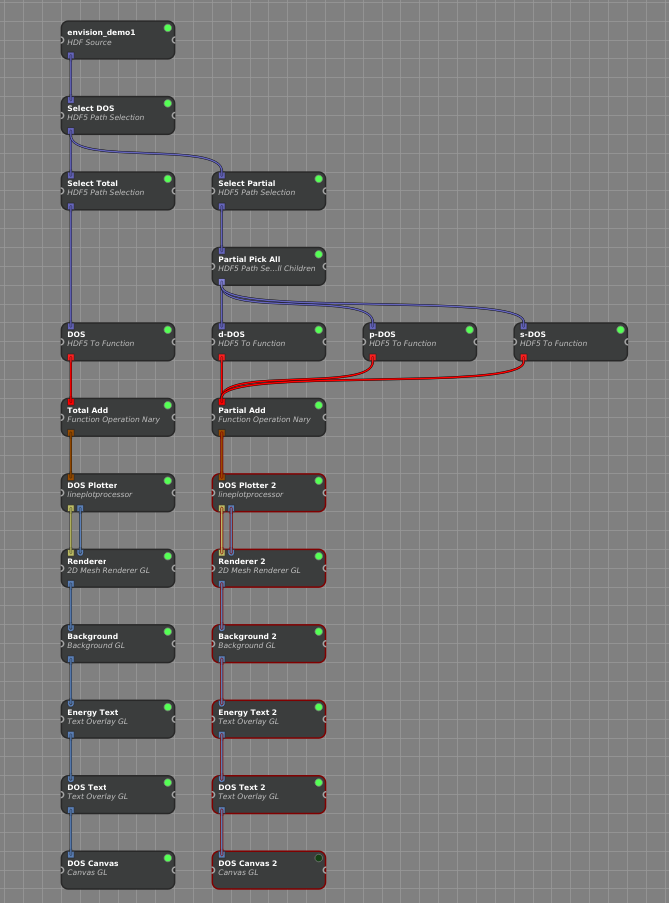
\includegraphics[scale=0.4]{screenshot_dos_network_Cu_1_10.png}
    \caption{Network for visualisation of total and partial DOS for Cu.}
    \label{fig:network_dos}
\end{figure}

\subsection{Interconnected networks}
Descriptions and examples of the python scripts generating interconnected networks can be seen below.

\subsubsection{Unit cell and charge}
In the Python editor in Inviwo, the user can choose to generate a visualisation of unitcell and charge by opening the folder \textit{scripts} and running the file \textit{unitcellAndCharge.py}.

\subsubsection{Unit cell and ELF}
In the Python editor in Inviwo, the user can choose to generate a visualisation of unitcell and ELF by opening the folder \textit{scripts} and running the file \textit{unitcellAndElf.py}. Figure \ref{fig:sammankoppling} shows what this can look like.

\begin{figure} [H]
\centering
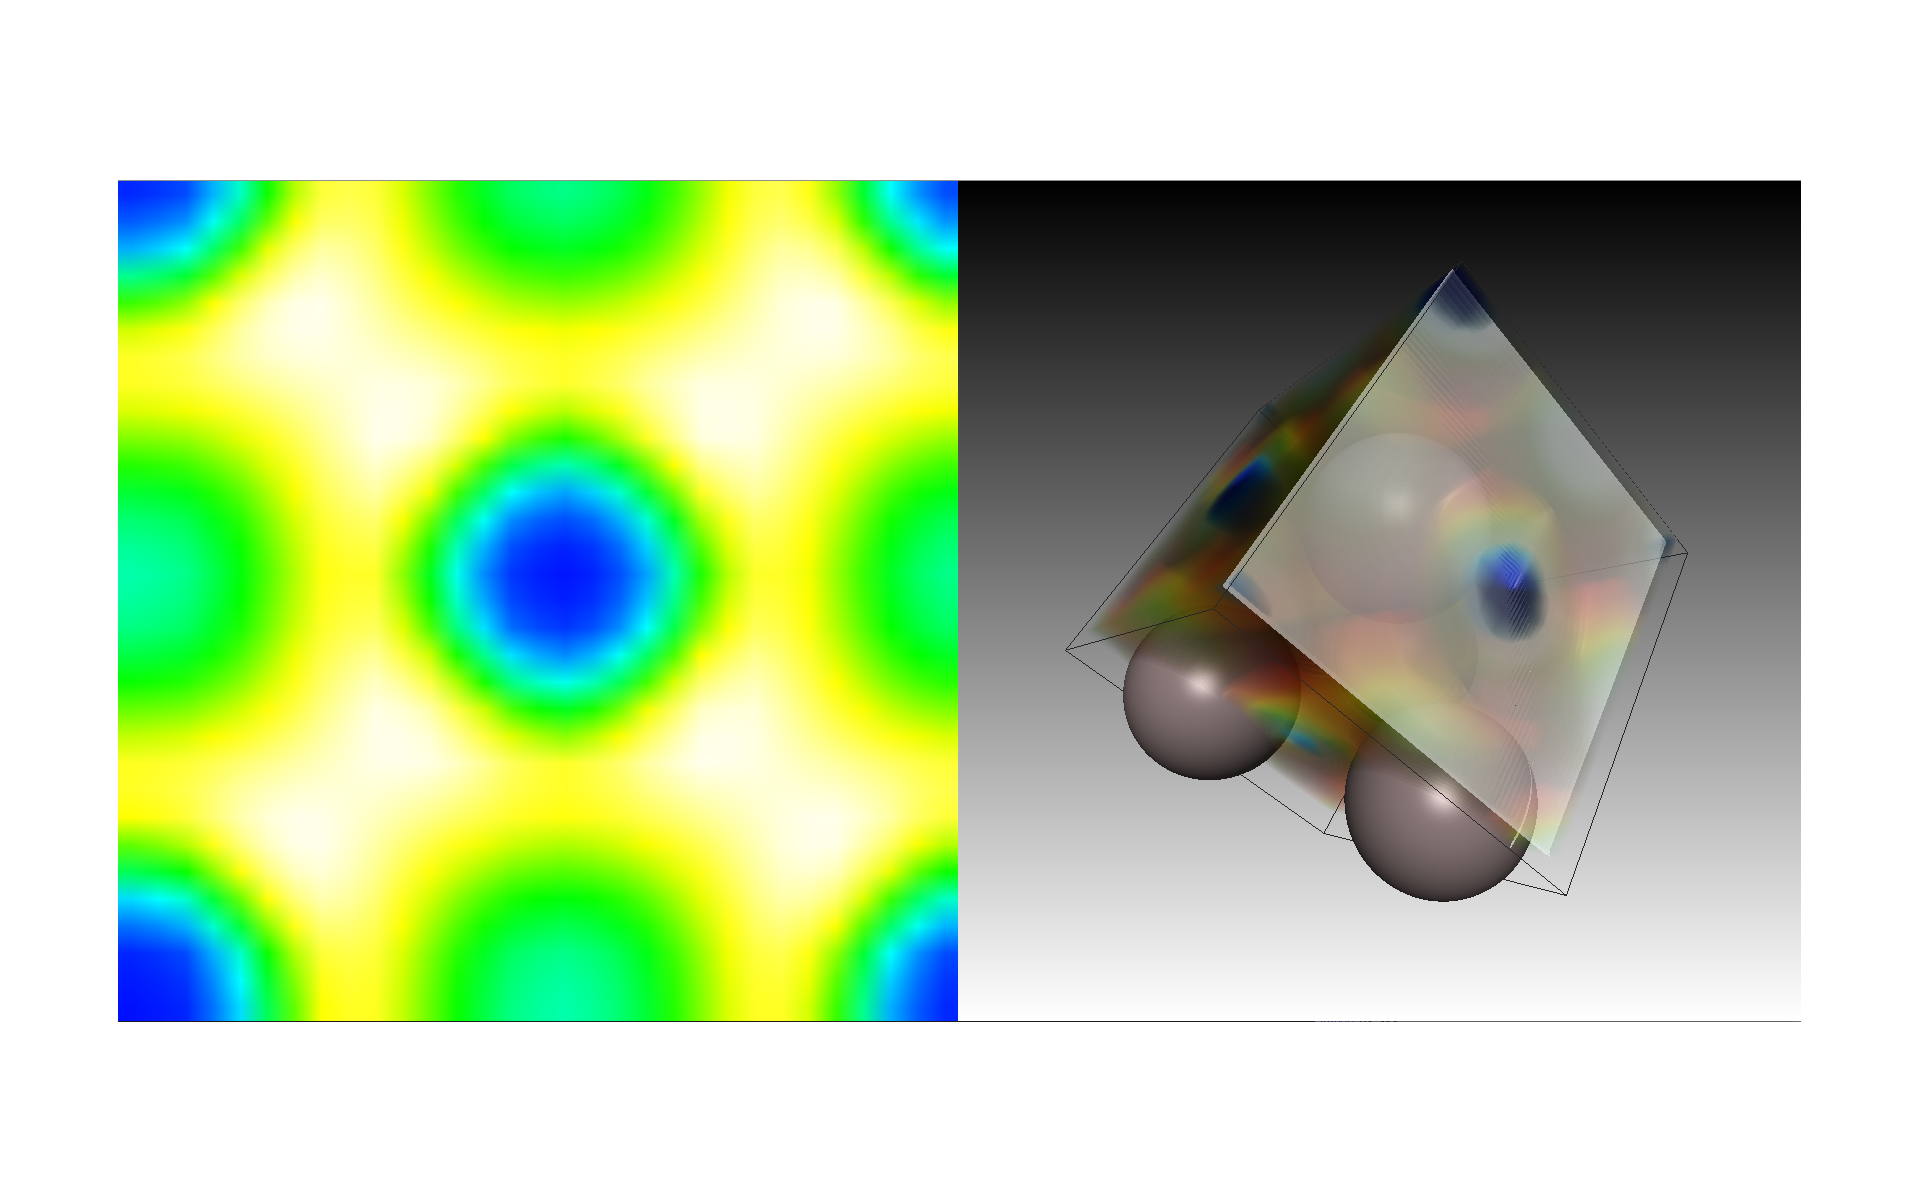
\includegraphics[scale=0.25]{screenshot_sammankoppling_Al.png}
\caption{Unit cell and ELF data for aluminum visualised side by side, with volume raycasting and slice function.}
\label{fig:sammankoppling}
\end{figure}

\subsubsection{Unit cell and DOS}
\label{ch:unitcell_dos}
In the Python editor in Inviwo, the user can choose to generate a visualisation of unitcell and density of states by opening the folder \textit{scripts} and running the file \textit{unitcellAndDos.py}. Here the user can pick an atom for which to show partial DOS by clicking on the desired atom in the unit cell. See figure \ref{fig:unitcell_dos} for an example of what this can look like.

\begin{figure}[H]
    \centering
    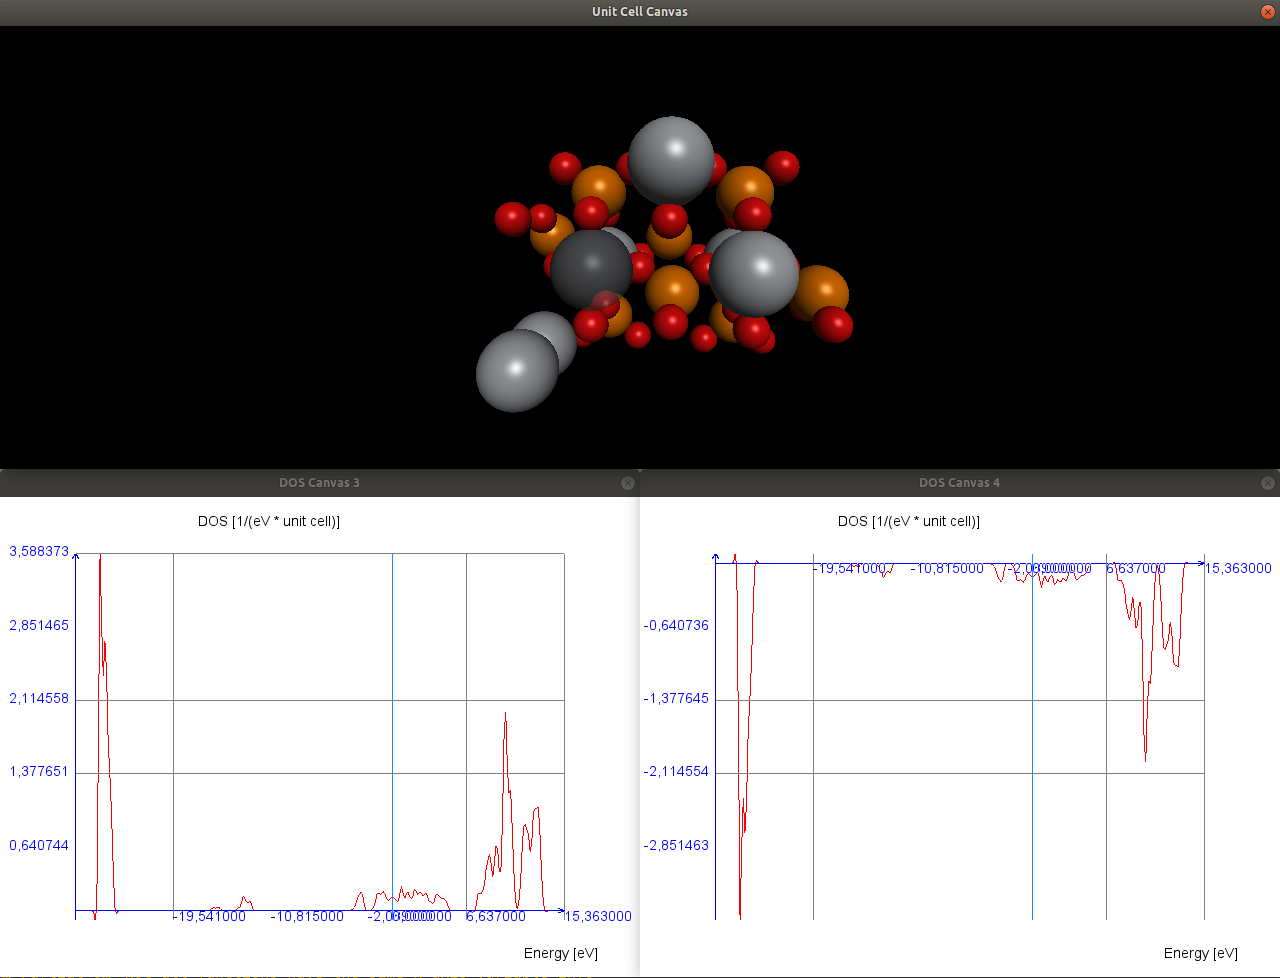
\includegraphics[scale=0.4]{screenshot_unitcell_dos.png}
    \caption{Visualisation of unit cell data and partial DOS of a titanium atom. The two graphs show DOS for electron spin up and electron spin down.}
    \label{fig:unitcell_dos}
\end{figure}


\newpage
\addcontentsline{toc}{section}{Referenser}
\printbibliography{}

\begin{appendices}

\section{Licens}
\label{ref:licens}
 Creative Commons Legal Code

CC0 1.0 Universal

    CREATIVE COMMONS CORPORATION IS NOT A LAW FIRM AND DOES NOT PROVIDE
    LEGAL SERVICES. DISTRIBUTION OF THIS DOCUMENT DOES NOT CREATE AN
    ATTORNEY-CLIENT RELATIONSHIP. CREATIVE COMMONS PROVIDES THIS
    INFORMATION ON AN ``AS-IS'' BASIS. CREATIVE COMMONS MAKES NO WARRANTIES
    REGARDING THE USE OF THIS DOCUMENT OR THE INFORMATION OR WORKS
    PROVIDED HEREUNDER, AND DISCLAIMS LIABILITY FOR DAMAGES RESULTING FROM
    THE USE OF THIS DOCUMENT OR THE INFORMATION OR WORKS PROVIDED
    HEREUNDER.

Statement of Purpose

The laws of most jurisdictions throughout the world automatically confer
exclusive Copyright and Related Rights (defined below) upon the creator
and subsequent owner(s) (each and all, an ``owner'') of an original work of
authorship and/or a database (each, a ``Work'').

Certain owners wish to permanently relinquish those rights to a Work for
the purpose of contributing to a commons of creative, cultural and
scientific works ("Commons") that the public can reliably and without fear
of later claims of infringement build upon, modify, incorporate in other
works, reuse and redistribute as freely as possible in any form whatsoever
and for any purposes, including without limitation commercial purposes.
These owners may contribute to the Commons to promote the ideal of a free
culture and the further production of creative, cultural and scientific
works, or to gain reputation or greater distribution for their Work in
part through the use and efforts of others.

For these and/or other purposes and motivations, and without any
expectation of additional consideration or compensation, the person
associating CC0 with a Work (the "Affirmer"), to the extent that he or she
is an owner of Copyright and Related Rights in the Work, voluntarily
elects to apply CC0 to the Work and publicly distribute the Work under its
terms, with knowledge of his or her Copyright and Related Rights in the
Work and the meaning and intended legal effect of CC0 on those rights.

1. Copyright and Related Rights. A Work made available under CC0 may be
protected by copyright and related or neighboring rights ("Copyright and
Related Rights"). Copyright and Related Rights include, but are not
limited to, the following:

  i. the right to reproduce, adapt, distribute, perform, display,
     communicate, and translate a Work;
     
 ii. moral rights retained by the original author(s) and/or performer(s);
 
iii. publicity and privacy rights pertaining to a person's image or
     likeness depicted in a Work;
     
 iv. rights protecting against unfair competition in regards to a Work,
     subject to the limitations in paragraph 4(a), below;
     
  v. rights protecting the extraction, dissemination, use and reuse of data in a Work;
  
 vi. database rights (such as those arising under Directive 96/9/EC of the
     European Parliament and of the Council of 11 March 1996 on the legal
     protection of databases, and under any national implementation
     thereof, including any amended or successor version of such
     directive); and
     
vii. other similar, equivalent or corresponding rights throughout the
     world based on applicable law or treaty, and any national
     implementations thereof.

2. Waiver. To the greatest extent permitted by, but not in contravention
of, applicable law, Affirmer hereby overtly, fully, permanently,
irrevocably and unconditionally waives, abandons, and surrenders all of
Affirmer's Copyright and Related Rights and associated claims and causes
of action, whether now known or unknown (including existing as well as
future claims and causes of action), in the Work (i) in all territories
worldwide, (ii) for the maximum duration provided by applicable law or
treaty (including future time extensions), (iii) in any current or future
medium and for any number of copies, and (iv) for any purpose whatsoever,
including without limitation commercial, advertising or promotional
purposes (the "Waiver"). Affirmer makes the Waiver for the benefit of each
member of the public at large and to the detriment of Affirmer's heirs and
successors, fully intending that such Waiver shall not be subject to
revocation, rescission, cancellation, termination, or any other legal or
equitable action to disrupt the quiet enjoyment of the Work by the public
as contemplated by Affirmer's express Statement of Purpose.

3. Public License Fallback. Should any part of the Waiver for any reason
be judged legally invalid or ineffective under applicable law, then the
Waiver shall be preserved to the maximum extent permitted taking into
account Affirmer's express Statement of Purpose. In addition, to the
extent the Waiver is so judged Affirmer hereby grants to each affected
person a royalty-free, non transferable, non sublicensable, non exclusive,
irrevocable and unconditional license to exercise Affirmer's Copyright and
Related Rights in the Work (i) in all territories worldwide, (ii) for the
maximum duration provided by applicable law or treaty (including future
time extensions), (iii) in any current or future medium and for any number
of copies, and (iv) for any purpose whatsoever, including without
limitation commercial, advertising or promotional purposes (the
"License"). The License shall be deemed effective as of the date CC0 was
applied by Affirmer to the Work. Should any part of the License for any
reason be judged legally invalid or ineffective under applicable law, such
partial invalidity or ineffectiveness shall not invalidate the remainder
of the License, and in such case Affirmer hereby affirms that he or she
will not (i) exercise any of his or her remaining Copyright and Related
Rights in the Work or (ii) assert any associated claims and causes of
action with respect to the Work, in either case contrary to Affirmer's
express Statement of Purpose.

4. Limitations and Disclaimers.

 a. No trademark or patent rights held by Affirmer are waived, abandoned,
    surrendered, licensed or otherwise affected by this document.
    
 b. Affirmer offers the Work as-is and makes no representations or
    warranties of any kind concerning the Work, express, implied,
    statutory or otherwise, including without limitation warranties of
    title, merchantability, fitness for a particular purpose, non
    infringement, or the absence of latent or other defects, accuracy, or
    the present or absence of errors, whether or not discoverable, all to
    the greatest extent permissible under applicable law.
    
 c. Affirmer disclaims responsibility for clearing rights of other persons
    that may apply to the Work or any use thereof, including without
    limitation any person's Copyright and Related Rights in the Work.
    Further, Affirmer disclaims responsibility for obtaining any necessary
    consents, permissions or other rights required for any use of the
    Work.
    
 d. Affirmer understands and acknowledges that Creative Commons is not a
    party to this document and has no duty or obligation with respect to
    this CC0 or use of the Work.

\end{appendices}

\end{document} 
